\documentclass{article}


% if you need to pass options to natbib, use, e.g.:
%     \PassOptionsToPackage{numbers, compress}{natbib}
% before loading neurips_2023


% ready for submission
%\usepackage{neurips_2023}


% to compile a preprint version, e.g., for submission to arXiv, add add the
% [preprint] option:
    % \usepackage[preprint,nonatbib]{neurips_2023}


% to compile a camera-ready version, add the [final] option, e.g.:
    \usepackage[final,nonatbib]{neurips_2023}


% to avoid loading the natbib package, add option nonatbib:
    % \usepackage[nonatbib]{neurips_2023}


\usepackage[utf8]{inputenc} % allow utf-8 input
\usepackage[T1]{fontenc}    % use 8-bit T1 fonts
\usepackage{url}            % simple URL typesetting
\usepackage{booktabs}       % professional-quality tables
\usepackage{amsfonts}       % blackboard math symbols
\usepackage{nicefrac}       % compact symbols for 1/2, etc.
\usepackage{microtype}      % microtypography
\usepackage{xcolor}         % colors
\usepackage{graphicx}  % for figures
\usepackage[font=small]{caption}

\usepackage{amsmath}  % for math symbols
\usepackage{amssymb} % for math symbols
\usepackage{pifont}  % for more symbols
\usepackage{tabularx}   % for tables
\usepackage{colortbl}  % table row colour
\usepackage{multirow}  % multi-row table
\usepackage{xspace}  % intelligent space after definitions
\usepackage{enumitem}  % unordered lists


\newcommand{\cmark}{\ding{51}}% checkmarks
\newcommand{\xmark}{\ding{55}}% crossmarks

\newcommand{\venue}[1]{{$_{\text{#1}}$}}  % venue 
\newcommand\dht[1]{\textcolor{gray}{#1}}  % gray text
\definecolor{Gray}{gray}{0.90}  % name color
\newcommand{\todo}[1]{\textcolor{red}{#1}}  % todo command

\def\ours{LSS\xspace}


\usepackage[pagebackref,breaklinks,colorlinks]{hyperref} % hyperlinks
\usepackage[capitalize]{cleveref}  % easy cross-referencing

\title{Language-based Action Concept Spaces Improve \\ Video Self-Supervised Learning}


\author{%
  Kanchana Ranasinghe \\
  Stony Brook University \\
  \texttt{kranasinghe@cs.stonybrook.edu} \\
  \And
  Michael Ryoo \\
  Stony Brook University \\
  \texttt{mryoo@cs.stonybrook.edu} \\
}


\begin{document}


\maketitle

\begin{abstract}
Recent contrastive language image pre-training has led to learning highly transferable and robust image representations. However, adapting these models to video domain with minimal supervision remains an open problem. We explore a simple step in that direction, using language tied self-supervised learning to adapt an image CLIP model to the video domain. A backbone modified for temporal modeling is trained under self-distillation settings with train objectives operating in an \textit{action concept space}. Feature vectors of various action concepts extracted from a language encoder using relevant textual prompts construct this space. A large language model aware of actions and their attributes generates the relevant textual prompts.
We introduce two train objectives, \textit{concept distillation} and \textit{concept alignment}, that retain generality of original representations while enforcing relations between actions and their attributes. Our approach improves zero-shot and linear probing performance on three action recognition benchmarks.
\end{abstract}

\section{Introduction}
\label{sec:intro}


Actions in videos are defined by individual objects, their relationships, and interaction \cite{Ryoo2006RecognitionOC,Aggarwal2011HumanAA}. Video self-supervised learning focuses on discovering representations aware of such action attributes directly from video content with no human supervision \cite{Chantry_SSLV}. Particularly in the case of videos, where manual human annotation can be both expensive and noisy, such self-supervised approaches are invaluable.
% and highly scalable with data.

A recent variant of self-supervision explores learning with loosely paired image-caption pairs, leading to highly transferable and robust representations such as CLIP \cite{radford2021clip}. These approaches obtain zero-shot performance often comparable to fully-supervised methods. However, their counterparts in the video domain \cite{xue2022clipvip, yan2022videococa, qian2022multimodal, ju2022prompting, rasheed2022fine, cheng2022vindlu,wang2021actionclip} do not exhibit the same generality. In fact, some approaches training CLIP on videos \cite{wang2021actionclip,ma2022xclip} perform subpar to image-CLIP under zero-shot settings (see \cref{lss_tbl:zeroshot}). 
% often lack such generality (e.g. \cref{lss_tbl:zeroshot})
Such behaviour can be attributed to lesser availability and more noisy nature of labelled (or paired caption) video datasets \cite{Chantry_SSLV}. This motivates exploration into self-supervised learning (SSL) techniques
that can learn from videos under less supervision while utilizing existing image CLIP \cite{radford2021clip} like representations. 
% be modified to while utilizing the existing strong image level representations from approaches like CLIP \cite{radford2021clip}. 
Existing state-of-the-art video SSL approaches \cite{Ran2021SVT,Tong2022VidMAE} learn highly transferable representations from videos, but combining these with image CLIP representations is not straightforward. In fact,  despite methods like SVT \cite{Ran2021SVT} being able to utilize image SSL representations \cite{caron2021emerging} for weight initialization to achieve better performance, using image CLIP representations instead for weight initialization leads to performance subpar to image CLIP (see \cref{lss_tbl:ablate_ssl}). 
This raises necessity for alternate video SSL approaches compatible with CLIP like image representations and is our key motivation.     

In this work, we explore self-supervised learning techniques that adapt image CLIP models \cite{radford2021clip} to video domain under entirely self-supervised settings, dependent on no form of video level labels or captions. Under this setting, natural language can still provide strong cues regarding attributes that compose an action category \cite{brattoli2020rethinking,xu2017transductive}. We leverage this idea to propose a novel \textit{language-based} self-supervised learning objective. Following a standard self-distillation and multi-view based SSL formulation \cite{caron2021emerging,Ran2021SVT}, we introduce language aligned feature spaces, \textit{action concept spaces}, where our SSL objectives operate. Large-language models (LLMs) \cite{brown2020language}, given their extensive world knowledge \cite{Zhao2023ASO,Naveed2023ACO}, serve as an ideal tool to generate necessary textual concepts for these spaces.   
We also introduce regularization suitable for our language aligned SSL objective to prevent collapse during training. Our resulting framework is termed \textit{Language-based Self-Supervision}, or LSS. 
% In this work, we explore self-supervised learning techniques that can adapt the representations of image CLIP models \cite{radford2021clip} to the video domain under entirely self-supervised settings, dependent on no form of video level labels or captions. Under this setting, natural language can still provide strong cues regarding attributes that compose an action category. Motivated by prior zero-shot action recognition work \cite{brattoli2020rethinking,xu2017transductive}, we leverage this idea to propose novel language-based self-supervised learning objectives, \textit{concept distillation} and \textit{concept alignment}. Large-language models (LLMs) \cite{brown2020language}, given their extensive world knowledge \cite{Zhao2023ASO,Naveed2023ACO}, serve as an ideal tool for generating necessary sets of language concepts related to actions.   
% Following a standard self-distillation and multi-view based SSL formulation \cite{caron2021emerging,Ran2021SVT}, we introduce language aligned feature spaces, \textit{action concept spaces}, where our SSL objectives operate. 
% We also introduce regularization suitable for our language aligned SSL objective to prevent collapse during training. Our resulting framework is termed \textit{Language-based Self-Supervision}, or \ours. 

In contrast to existing video self-supervised learning approaches \cite{Ran2021SVT,Tong2022VidMAE}, our proposed LSS retains and improves transferability of image CLIP representations much better (see \cref{lss_tbl:linear,lss_tbl:ablate_ssl}). Additionally, our language aligned learning framework allows direct zero-shot operation on downstream tasks. 
Moreover, unlike video CLIP methods with similar zero-shot capabilities \cite{xue2022clipvip, yan2022videococa, qian2022multimodal, ju2022prompting, rasheed2022fine, cheng2022vindlu,wang2021actionclip} that utilize per-video labels / captions for learning, our proposed LSS requires only videos for training. 

We summarize our key contributions as follows:
\begin{itemize}[leftmargin=2em,noitemsep,topsep=1.0ex,itemsep=-0.5ex,partopsep=0ex,parsep=1ex]
    \item Self-supervised learning paradigm capable of retaining and improving strengths of CLIP like image representations for video domain operation
    \item Video specific self-supervised learning objectives, namely \textit{concept distillation} and \textit{concept alignment}, that enforce relations between action categories and their visual attributes 
    \item Novel language-based video self-supervised learning framework operating zero-shot on downstream action classification tasks without requiring per-video labels / captions for training
    
\end{itemize}

Experiments on action recognition datasets showcase state-of-the-art performance for our learned representations under linear-probing, standard zero-shot, and transductive zero-shot settings. 
% HMDB-51 \cite{kuehne2011hmdb}, UCF-101 \cite{soomro2012ucf}, and Kinetics-400 \cite{kinetics400}
\section{Language Based Video Self-Supervised Learning}
\label{lss:related}

\bhdr{Self-Supervised Learning in Videos} was initially dominated by pretext tasks specific to the video domain \cite{mathieu2015deep, PatrauceanHC16, walker2016uncertain, pmlr-v37-srivastava15, Vondrick16a, vondrick2018tracking, Agrawal_2015_ICCV, Goroshin_2015_ICCV, DBLP:journals/corr/IsolaZKA15, Misra-2016-5596, 7410677, piergiovanni2020evolving}. Recently a shift to contrastive losses led to \cite{Feichtenhofer_large, han2019video, han2020self, qian2020spatiotemporal, hjelm2020representation, recasens2021broaden} with some variants focused on video specific view generation \cite{Huang_2021_ICCV, chen2021rspnet, Behrmann2021LongSV, Dave2021TCLRTC, Ran2021SVT}. An alternate direction has been masked auto-encoders \cite{Tong2022VidMAE}.
To the best of our knowledge, existing video self-supervised learning (SSL) approaches operate purely within the visual domain. By video SSL, we refer to methods that utilize only videos with no paired captions (or labels) for each video during training.
In contrast, our proposed LSS learns purely from videos in a self-supervised manner, integrating pre-trained language-image models to learn language aligned representations. 

\vspace{0.5em}


\bhdr{Zero-shot Action Recognition} began with manual attribute and feature selection \cite{liu2011recognizing,zellers2017zero, jain2015objects2action,gao2019know,gao2020learning} with later works utilizing action word embeddings \cite{brattoli2020rethinking,xu2017transductive}. The idea of connecting action categories with elaborate descriptions of those actions, within language embedding spaces \cite{chen2021erzsar,zhu2018ur} has been a next step and is closely related to our work. This idea is also explored in image domain to boost zero-shot performance \cite{menon2022visual}. While our work is inspired by such approaches, in contrast, we use relations between such actions and descriptions as self-supervised signals for learning. 
Recent image CLIP models \cite{radford2021clip,jia2021align} are another line of works achieving strong performance on some video classification tasks, with only single frame processing. Multiple approaches build on image CLIP \cite{radford2021clip} to learn video level representations \cite{wang2021actionclip, luo2022clip4clip, bain2022cliphitchhiker, lin2022evl, ma2022xclip, Kahatapitiya2023VicTRVT} under fully-supervised settings. While achieving strong performance on the training datasets, their zero-shot improvements over CLIP are minimal or even subpar (see \cref{lss_tbl:zeroshot}). Therein, LSS focuses on zero-shot performance under self-supervised settings while retaining (and improving) the generality of the representation space.

\vspace{0.5em}

\bhdr{Self-training} methods leverage pseudo-labels on unlabeled data \cite{mean_teacher,fixmatch,remixmatch} for supervised-fashion training. Recently they have been combined with CLIP models for zero-shot operation \cite{Li2022MaskedUS, Kahana2022ImprovingZM}. While inspired by such self-training approaches, our proposed LSS differs in its continuous feature space self-distillation, language-based relations enforcing, video domain operation, and cross-dataset transfer for zero-shot operation. 

\vspace{0.5em}

\bhdr{Adapting image-CLIP models to video} under fully-supervised settings has gathered much interest \cite{xue2022clipvip, yan2022videococa, qian2022multimodal, ju2022prompting, rasheed2022fine, cheng2022vindlu}. Expanding backbones for temporal modeling, multi-modal fusion, secondary training objectives, partial parameter updates, and scaling-up data are key ideas explored \cite{Kahatapitiya2023VicTRVT,cheng2022vindlu}. In contrast, LSS is a first to operate under self-supervised settings using no video annotations. 

\vspace{0.5em}

\bhdr{Contemporary work} in \cite{Lin2023MAtchEA} adapts image CLIP features to video tasks label free similar to our work. ViFi-CLIP \cite{Rasheed2022FinetunedCM} introduces zero-shot action recognition benchmarks and similarly adapts CLIP to videos retaining generality. Using LLMs for action recognition is also explored in \cite{Hanu2023LanguageAT}. 
\section{Language-based Self-Supervision (LSS)}
\label{lss_sec:method}
In this section, we present our proposal, Language-based Self-Supervision (LSS). The generality and robustness of shared image-language representation spaces such as that of CLIP \cite{radford2021clip} allow interesting manipulations of visual representations using language. We explore such manipulations under the setting of visual self-supervised learning focusing on video understanding. Self-supervised objectives can operate within a latent space constructed with language, retaining language alignment of learned visual representations. This allows better interpretability of representations as well as zero-shot inference. 
We discuss the four key components of our approach: backbone architecture, concept distillation objective, modifications to avoid collapse, and concept alignment objective.

\begin{figure}
\includegraphics[width=\textwidth]{src/1_LSS/figures/arch1.pdf}
\vspace{-1.5em}
\caption[Architecture Overview]{\small
\textbf{Architecture Overview:}
Our overall setup contains three components: visual teacher model (green), visual student model (red), and language model (blue). We utilize the text encoder of CLIP as our language model and extract \textit{concept vectors} relevant to action labels and descriptions of those actions. A visual encoder (containing a space-time backbone) is partially initialized with CLIP's visual encoder and used to obtain sample specific features. Generated concept vectors are used to project these features to a \textit{concept space} where our proposed \textit{concept distillation} and \textit{concept alignment} losses are applied.
}
\label{lss_fig:arch}
\end{figure}

\subsection{Backbone Architecture}
\label{lss_subsec:arch}
Our approach introduces a \textit{text classifier} to self-distillation based SSL works \cite{caron2021emerging, Ran2021SVT}, in place of the projector network.
% Our approach builds over self-distillation based SSL works \cite{caron2021emerging, Ran2021SVT} introducing a \textit{text classifier} in place of the projector network. 
Given a data sample $x$, let $x_1, x_2 \in \mathbb{R}^{(C,T,H,W)}$ be two augmented views generated using video specific transformations following \cite{Ran2021SVT}, where $C=3, T=8, H=W=224$ are channel, time, and spatial dimensions respectively. 

\textbf{Visual Encoder:}
A visual encoder, $\theta_v$, processes $x_i$ to produce feature $f_i \in \mathbb{R}^{768}$. We utilize the pre-trained image encoder of CLIP \cite{radford2021clip} expanded for temporal modelling using factorized space-time attention. The vision transformer variant of CLIP is selected to allow our factorized space-time attention. In particular, we use ViT-B/16 architecture for the the image encoder, in which for a given augmented view with $H=W=224$ and $T=8$, each transformer block processes 8 temporal and 196 spatial tokens separately in sequential order, and the embedding dimension of each token is $\mathbb{R}^{768}$. 
In addition to the input tokens from the data sample, one classification token \cite{devlin2018bert, dosovitskiy2020image} serves as the final feature vector output by the network, namely $f_i$, which is common to the CLIP image encoder. This classification token is inflated and processed suitably following \cite{bertasius2021timesformer} to accommodate our modifications for factorized space-time attention.  We follow \cite{bertasius2021timesformer} to zero-initialize additional time-attention parameters, achieving outputs identical to the pre-trained CLIP image encoder at start of training. 

\textbf{Text Classifier:}
Inspired by \cite{wu2022text4vis}, a set of $n$ language embeddings extracted from the CLIP text encoder, $\theta_t$, are used to construct the weight parameter of a linear layer (with no bias term), which we call our text classifier, $\theta_c$. The role of this text classifier is to project visual features $f_i$ to a vector space defined by those $n$ embeddings, producing $\tilde{f}_i \in \mathbb{R}^n$. Next we discuss these vector spaces (referred to as action concept spaces) and the text classifier module in detail.

\begin{figure}
\centering
\includegraphics[width=0.99\textwidth]{src/1_LSS/figures/concept_space1.pdf}
\vspace{-0.5em}
\caption[Concept Space Illustration]{\small
\textbf{Concept Spaces:}
We illustrate a toy concept space constructed with the three action concepts: run, swim, and walk. In this example, the text classifier projects visual feature $f_i$ into the 3-dimensional toy concept space to produce $\tilde{f}_i$. 
}
\label{lss_fig:cs}
\end{figure}

\subsection{Action Concept Spaces}
\label{subsec:concept_space}
Self-supervised learning approaches following exponential moving average (EMA) based self-distillation \cite{grill2020bootstrap,caron2021emerging,Ran2021SVT} utilize a projector network (MLP) to operate in a higher dimensional feature space. This is expected to minimize train-test domain gaps, handle noisy positive sample pairs, and better discriminate nuanced feature differences \cite{Balestriero2023ACO}. Focused on these notions, we propose an alternate \textit{concept space} composed of a set of basis vectors defined by language-based action concepts. Our language-based self-supervision objectives operate within such concept spaces.

\textbf{Concept Spaces:}
Building off the assumption that text encoder features capture subtle differences between distinct actions categories, we hypothesize that necessary nuanced distinctions between these actions will be better captured in our proposed concept spaces. The defining parameters of concept spaces are their basis vectors, $b_i$. Normalized embeddings (extracted from text encoder, $\theta_t$) of various natural language captions ($c_i$) relevant to action categories are used as these basic vectors. 
%
\begin{align}
    b_i &= {\theta_t(c_i)} \left. \right/ {||\theta_t(c_i)||^2_2} \\
    \mathbf{b} &= [b_1, b_2, ... \ b_n]^T \text{ ; } \mathbf{b} \in \mathbb{R}^{(n, d)} 
\end{align}
%
Note that these basis vectors are not necessarily orthogonal. As illustrated in \cref{lss_fig:cs}, a single set of basis vectors, $\mathbf{b}$, defines one action concept space.
We define two sets of basic vectors: action category vectors and action description vectors. Action category vectors relate to a single action label which is converted to a caption using textual prompting following \cite{radford2021clip}. Action description vectors are averaged embeddings of multiple descriptions and visual characteristics relevant to individual action categories. These two distinct sets of basic vectors lead to two distinct concept spaces which we name \textit{category concept space} and \textit{description concept space} respectively.  

\textbf{Category Concept Space:}
We explore 3 different strategies to construct the category concept space. The base setup uses action labels from Kinetics-400 \cite{kinetics400}, UCF-101 \cite{soomro2012ucf}, and HMDB-51 \cite{kuehne2011hmdb} datasets, leading to a set of 530 (400 + 101 + 51, ignoring overlaps) basis vectors. Our next goal of connecting LLMs and their action awareness occurs in the second two strategies. We utilize LLMs \cite{brown2020language} and visual-LLMs \cite{liu2023llava} to extract large sets of action category labels. While we explore this idea of expanding the basis vector set with LMM based additional action labels in \cref{sec:experiments}, the base setup containing a modest 530 categories was sufficient to improve downstream task performance.

\textbf{Description Concept Space:}
This space is constructed conditioned on the previous category concept space. For each action label used in the latter, we extract 4 distinct descriptions and a set of visual characteristics relevant to that action label using a large language model (LLM). The role of the LLM is to inject its world knowledge (i.e. awareness on videos, actions, and their attributes) into our learned representations during self-supervised learning. 
In detail, we prompt GPT-3 \cite{brown2020language} to generate such descriptions and characteristics using procedure outlined in \cref{app:gpt_prompting}. We highlight that GPT-3 is used here as an intelligent LLM containing world knowledge on videos and actions, in order to create natural language descriptions for given action category labels. 
The textual outputs generated for each action label are processed by our text encoder to produce multiple embeddings for a single action label. These embeddings are averaged to produce the corresponding basis vector for the description concept space. Note how this leads to a common dimensionality between the two concept spaces as well as one to one correspondences between the basic vectors of the spaces, which we leverage in our self-supervision objectives. 


\subsection{Concept Distillation}
\label{subsec:cd}
We now describe our primary self-supervised learning objective, concept distillation. Standard multi-view based self-supervision enforces a network to encode the common information between two augmented (distorted) views of a data sample \cite{Balestriero2023ACO}. This common information can be considered as the augmentation invariant signal present in the original data sample \cite{Balestriero2023ACO,Bardes2021VICRegVR}. In the case of self-distillation based approaches \cite{caron2021emerging,Ran2021SVT}, a higher dimensional feature space is utilized to enforce the self-supervision objectives. Instead, we propose to use action concept spaces as an alternative.
% , focusing on the case of video based self-supervision. 

Proposed concept distillation depends on an action concept space and visual video features aligned to the basis vectors of that space. Given our visual features $f_i \in \mathbb{R}^d$, we obtain projected $\tilde{f}_i \in \mathbb{R}^n$ as,  
%
\begin{align}
    % \mathbf{b} &= [b_1, b_2, ... \ b_n]^T \text{ ; } \mathbf{b} \in \mathbb{R}^{(n, d)} \notag \\
    \tilde{f}_i &= \mathbf{b} \ (\left. f_i \right/ ||f_i||^2_2) 
    = [b_1 \cdot f_i', b_2 \cdot f_i', ... \ b_n \cdot f_i']^T 
\end{align}
\textbf{Similarity Calculation: }
Projecting normalized visual video features to a concept space corresponds to calculating the dot-product similarity with each basic vector of the concept space. The projected vector $\tilde{f}_i$ can be viewed as a similarity \textit{score distribution} across all basis vectors of the concept space. Inspired by \cite{wu2022text4vis}, we implement this similarity calculation as a linear layer with weight matrix $\mathbf{b}$ and bias terms zero. We refer to this layer as the \textit{text classifier}. Similar to \cite{wu2022text4vis}, our text classifier remains frozen (no parameter updates), but in our case, this is to retain the original language distribution. 

\textbf{Concept Distillation Objective:}
Viewing projected features for two augmented views of a single video as score distributions, we argue that the underlying signal of the original video would relate to a unique score distribution to which score distributions of each view should be similar. Therein, following our EMA teacher based self-distillation setup (see \cref{lss_subsec:arch} for details), we enforce the score distribution to be consistent across views. 
Given two views $x_1, x_2$ of a single video, our teacher and student visual encoders process them respectively to produce $f_1, f_2$. The text classifier projects these to concept space, producing score distributions $\tilde{f}_1, \tilde{f}_2$. We obtain our objective, $\mathcal{L}_{\text{CD}}$ as:  
 %
 \begin{align}
    \label{eq:softmax}
    \hat{f}_i[k] &= \frac{\operatorname{exp}(\tilde{f}_i[k] / \lambda_i)}
                      {\sum_{j=1}^{n} \operatorname{exp}(\tilde{f}_i[j]/ \lambda_i) } \\
    \label{eq:weight}
    w_s &=  \operatorname{max}(\hat{f}_1) \\
    \label{eq:loss_cd}
    \mathcal{L}_{\text{CD}}(\tilde{f}_1, \tilde{f}_2) &= - w_s \cdot \sum_{j=1}^{n} \hat{f}_1[j] \operatorname{log} \hat{f}_2[j] 
 \end{align}
 %
The teacher and student score distributions, $\tilde{f}_1, \tilde{f}_2$, are softmax normalized in \cref{eq:softmax}, with temperature terms $\lambda_1=0.1, \lambda_2=1$ for sharpening only the teacher score distribution. A significance score $w_s$ is calculated for each sample in \cref{eq:weight}. In the softmax normalized teacher score distribution ($\hat{f}_1$), the maximum value is high when peaked at a single action concept and low when peaked at multiple action concepts. Considering the noisy nature of multi-peak teacher score distributions, we utilize $w_s$ to minimize their overall effect during training. Our overall $\mathcal{L}_{\text{CD}}$ is thus implemented as in \cref{eq:loss_cd}.   

\textbf{Distinct Concept Spaces:} Given the two distinct action concept spaces defined in \cref{subsec:concept_space}, we utilize two parallel text classifiers to implement each, and obtain two score distributions, one for each concept space. Defining score distributions $\tilde{f}_i^C, \tilde{f}_i^D$ for category and description concept spaces respectively, we apply our $\mathcal{L}_{\text{CD}}$ on each pair separately to obtain two losses $\mathcal{L}_{\text{CD}}^{\text{X}}$ for 
{\small X$\in$\{C,D\}} as:
%
\begin{align}
    \mathcal{L}_{\text{CD}}^{\text{X}} = \mathcal{L}_{\text{CD}}(\tilde{f}_1^{\text{X}}, \tilde{f}_2^{\text{X}})
\end{align}
%
We highlight how our concept spaces implemented as text classifiers are maintained intact by freezing the text classifier during training. This allows our approach to perform direct zero-shot inference, making concept distillation additionally advantageous over standard video SSL techniques. 


\subsection{Uniform Distribution Prior}
\label{subsec:udp}
Avoiding collapse is a key concern in SSL methods \cite{caron2021emerging,Ran2021SVT,Balestriero2023ACO} and recent self-distillation based approaches utilize feature sharpening and centering operations to avoid collapse \cite{caron2021emerging,Ran2021SVT}. While we similarly perform sharpening operations on the teacher outputs, given the nature of our action concept space, performing a learned vector mean subtraction based centering operations can break the meaningful structure of score distributions. Instead, we enforce a uniform distribution prior on the expected score distribution over the entire training dataset. The centering operation proposed in \cite{caron2021emerging} acts similarly pushing representations towards a uniform distribution while the sharpening operation counters its effect. We approximate expectation over the dataset as a moving average of mean score distributions at each train iteration and the uniform prior is enforced as: 
%
\begin{align}
    \hat{f}_{\text{MA}}^{\text{X}} &= \tau \cdot \hat{f}_2^{\text{X}} + (1 - \tau) \cdot \hat{f}_{\text{MA}}^{\text{X}} \\
    \label{eq:up}
    \mathcal{L}_{\text{UP}}^{\text{X}} &= - \frac{1}{n} \sum_j \operatorname{log} \hat{f}_{\text{MA}}^{\text{X}}[j]
\end{align}
%
where the hyper-parameter $\tau=0.5$ is fixed during training. We highlight that $\mathcal{L}_{\text{UP}}$ is necessary for convergence with concept distillation and is added to the concept distillation objective, $\mathcal{L}_{\text{CD}}^{\text{X}}$. 

%\begin{alignat}{2}
%	x + y &= 5  &\quad&\text{first equation} \\
%	2x - y &= 1  &&\text{second equation}
%\end{alignat}


\subsection{Concept Alignment}
Aligning action category labels and their descriptions or attributes within some embedding space has been explored in video SSL under multiple settings \cite{chen2021erzsar,zhu2018ur}. Motivated by these promising results, we explore how such alignment can be integrated to improve our framework with \emph{concept spaces}. In \cref{subsec:concept_space}, we define two distinct action concept spaces constructed from category labels and detailed category descriptions respectively. We hypothesize that explicit alignment of video features between these two spaces based on their one to one relationship can learn additional information. Therein, we introduce our concept alignment objective, $\mathcal{L}_{\text{CA}}$, as follows:
%
\begin{align}
    \mathcal{L}_{\text{CA}} = \mathcal{L}_{\text{CD}}(\tilde{f}_1^{\text{C}}, \tilde{f}_2^{\text{D}}) + \mathcal{L}_{\text{CD}}(\tilde{f}_1^{\text{D}}, \tilde{f}_2^{\text{C}})
\end{align}
%
\textbf{Overall SSL Objective:}
Reusing $\mathcal{L}_{\text{CD}}$ from \cref{eq:loss_cd}, we match score distributions across our two concept spaces instead of within a single concept space. $\mathcal{L}_{\text{CD}}(\tilde{f}_1^{\text{C}}, \tilde{f}_2^{\text{D}})$ aligns student description score distribution $\tilde{f}_2^{\text{D}}$ to teacher category score distribution $\tilde{f}_1^{\text{C}}$ while $\mathcal{L}_{\text{CD}}(\tilde{f}_1^{\text{C}}, \tilde{f}_2^{\text{D}})$ aligns student category score distribution $\tilde{f}_2^{\text{C}}$ to teacher description score distribution $\tilde{f}_1^{\text{D}}$. Combining all terms, we obtain:
% This leads to our overall self-supervised training objective:
%
\begin{align}
\label{eq:overall}
\mathcal{L} = (\mathcal{L}_{\text{CD}}^\text{C} + \mathcal{L}_{\text{UP}}^\text{C}) + (\mathcal{L}_{\text{CD}}^\text{D} + \mathcal{L}_{\text{UP}}^\text{D}) + \mathcal{L}_{\text{CA}}
\end{align}


\subsection{Concept Space Variants}
Our baseline concept space (described in \cref{subsec:concept_space}) utilizes labels from three standard video datasets (Kinetics-400, UCF-101, HMDB-51). However, we want to ensure scalability with more data and no label leakage to downstream evaluation tasks. With this goal, we propose 2 additional variants of action concept spaces tagged LSS-B and LSS-C. These variants do not use any form of ground truth textual labels from datasets. Moreover, they leverage the world awareness (i.e. knowledge on videos and actions) of LLMs to generate extensive action categories. Our baseline setup is hereafter referred as LSS-A.  

For LSS-B, we use GPT-3 \cite{brown2020language} to generate a large set of action labels. We first prompt GPT to categorize all common human actions / activities into 20 groups. For each group, we again ask GPT to generate at least 100 visually diverse action categories. These are all collected to create a set of 2000 action labels. We then use projections of these labels in CLIP text-encoder representation space to eliminate labels of high semantic similarity (spectral clustering in feature space from \cite{ranasinghe2022perceptual} to identify similar features), achieving 1000 diverse action categories. So our 1000 action categories for LSS-B are generic, not tied to any of our training datasets, and scalable with more data.

For LSS-C, we generate a label set using only videos from the training dataset. We use PCA based clustering to identify 2000 representative videos from a randomly sampled subset (50,000) of our training dataset and then use image-captioning models (LLaVa \cite{liu2023llava}) on video center frames to generate a diverse set of 2000 action labels. This is further reduced to 500 eliminating labels that are similar in feature space of the CLIP text encoder. In this case, our generated labels are tied to the training dataset, but uses no textually annotated category labels. We use only the videos (and an image-to-text captioning model) to generate our label set, still resulting in a scalable framework.

Note that each of these alternate strategies relates to construction of our category concept space. Given the selected set of textual category labels of this space, the description concept space is constructed in the same common way (as described in \cref{subsec:concept_space}).  We also reiterate that LSS-B and LSS-C variants use no category information from train / test datasets. 


% Experiments Section
% User study data - single source of truth (DRY!)
% Study parameters
\newcommand{\NumParticipants}{41}

% Win rates
\newcommand{\OursQOne}{70}
\newcommand{\ATIQOne}{24}
\newcommand{\ReVideoQOne}{1}
\newcommand{\GWTFQOne}{5}

\newcommand{\OursQTwo}{71}
\newcommand{\ATIQTwo}{24}
\newcommand{\ReVideoQTwo}{2}
\newcommand{\GWTFQTwo}{3}

\newcommand{\OursQThree}{69}
\newcommand{\ATIQThree}{25}
\newcommand{\ReVideoQThree}{1}
\newcommand{\GWTFQThree}{5}

% Helper to convert percentage to decimal for plots
\newcommand{\pct}[1]{\fpeval{#1/100}}


\section{Results}
\label{sec:experiments}

\subsection{Implementation Details}

We use CogVideoX-5B~\cite{cogvideox2024} as our base text-to-video model for both the finetuned counterfactual video generation model and the V2V editing model.
Training was conducted on 8 H100 GPUs for one week using standard latent diffusion training with L2 loss.
We set $\Fframes = 49$,
with input resolution of $480 \times 720$ pixels,
corresponding to latent dimensions of $60 \times 90$.
We use $\Nblobs$ varying between 1 and 64 during training and set the control branch depth appropriately.
We use a learning rate of $10^{-4}$ and a dataset size of $100,000$ videos,
for $15,000$ iterations with an effective batch size of $32$.
We use an internal video dataset with 500,000 samples.
%\todo{fill number of samples}


\begin{comment}

USER STUDY
We conducted a user study to evaluate out algorithm.
We compared against ATI [cite], which is based on a newer base model WAN2.1 14B and operates on first-frame+motion-control-to-video
We manually created 20 videos
We had 10 participants
We asked them Q1: "Which video better preserves the input video's content?"
and Q2: "Which video better reflects the desired motion?"
and Q3: "Which video is overall a better edit of the input video?"

The results are in table TABLE1

TABLE1
	User Study
	[Ours] [ATI]
Q1: 70%    30%
Q2: 70%    30%
Q3: 70%    30%
[Caption: Users prefred ours yadda yadda]


QUANTITIVE EVALUATION:

We also created a qunantitative evaluation where we use photometric losses to gauge how good ours is against ATI
We created a dataset of 100 videos. We need to get counterfactual / ground truth pairs, so for each video we create an input and ground truth video as follows:
[potentially choose different variable names if it makes it more coherent] Given a test video v, we split v in the middle temporally to get v0 and v1. We then reverse v1 to get v1', so now the end of v0 is the start of v1'. We use v0 as the input video, and then choose 25 random points in that video the same way we do during training [ you can give tiny detail with better notation here]
For these 100 videos, we chose videos that have content exposed in the middle of the video that is not visible in the first frame, by choosing videos where there is a significant number of points that when tracked from the middle frame bidirectionally go missing in the first and last frames. [maybe we'll give again, a tiny equation here with notation - but only if you're confident you're doing it right]
For each algorithm we compare algo(v0) vs v1 using L2 loss on every frame.

TABLE1
	Photometric Loss
	[Ours] [ATI]
L2: .2    .5
[caption: ours had better photometric losses yadda yadda]

\end{comment}

% Additional macros for experiments
\newcommand{\Vtest}{V_{\text{test}}}     % test video
\newcommand{\Vzero}{V_0}                 % first half of test video  
\newcommand{\Vone}{V_1}                  % second half of test video
\newcommand{\Voneprime}{V_1'}            % reversed second half
% \newcommand{\Lphotometric}{\mathcal{L}_{\text{photo}}} % photometric loss (removed)
\newcommand{\Ntest}{N_{\text{test}}}     % number of test videos
\newcommand{\Npoints}{N_{\text{points}}} % number of tracking points for evaluation


We evaluate our motion editing approach through user studies and quantitative metrics, comparing against state-of-the-art motion control methods. %Details of how these baselines are implemented can be found in the appendix.

%\TODO{Explain how each baseline algorithm (ATI, ReVideo, Go-with-the-Flow, MotionPrompting) was implemented to work with our evaluation framework and track inputs. ---- PUT THAT IN APPENDIX }

\subsection{User Study}

We conducted a user study comparing our method against three baselines: ATI~\cite{ati},
a trajectory-guided image-to-video method based on WAN 2.1~\cite{wan};
ReVideo~\cite{revideo2024};
and Go-with-the-Flow (GWTF)~\cite{gowiththeflow2025}.
We manually created 20 test videos spanning diverse scenarios including object motion editing,
camera motion changes,
and complex scenes with multiple moving elements. \NumParticipants{} participants compared all four methods using the interface shown in the Supplementals,
selecting the best video for each of three questions per test case:
\begin{itemize}
    \item \textbf{Q1:} ``Which video better preserves the input video's content?''
    \item \textbf{Q2:} ``Which video better reflects the desired motion?''
    \item \textbf{Q3:} ``Which video is overall a better edit of the input video?''
\end{itemize}


\begin{table}[h]
\centering
\small
\begin{tabular}{l|cccc}
\hline
Question & Ours & ATI & ReVideo & GWTF \\
\hline
Q1: Content ($\uparrow$) & \textbf{\OursQOne\%} & \ATIQOne\% & \ReVideoQOne\% & \GWTFQOne\% \\
Q2: Motion ($\uparrow$) & \textbf{\OursQTwo\%} & \ATIQTwo\% & \ReVideoQTwo\% & \GWTFQTwo\% \\
Q3: Overall ($\uparrow$) & \textbf{\OursQThree\%} & \ATIQThree\% & \ReVideoQThree\% & \GWTFQThree\% \\
\hline
\end{tabular}
\caption{\textbf{User study win rates across all methods.}
Participants selected the best video for each question.
Our method consistently wins across all evaluation criteria.}
\label{tab:user_study}
\end{table}

Table~\ref{tab:user_study} show that users consistently ranked our method highest across all questions,
with win rates around 70\% compared to 25\% for ATI and less than 5\% for ReVideo and GWTF,
demonstrating superior content preservation and motion control.

\subsection{Quantitative Evaluation}

We developed a quantitative evaluation protocol using photometric reconstruction error to assess motion editing quality. 

\subsubsection{Dataset Construction}

We curated a dataset of $\Ntest = 100$ test videos using the following protocol.
Given a source video $\Vtest$ of length $\Ffull$ frames,
we split it temporally at the midpoint to obtain $\Vzero = \Vtest\left[1:\Ffull/2\right]$ and $\Vone = \Vtest\left[\Ffull/2:\Ffull\right]$.
We then create the counterfactual input by temporally reversing $\Vone$ to get $\Voneprime$,
ensuring temporal continuity between $\Vzero$ and $\Voneprime$ (i.e., the last frame of $\Vzero$ matches the first frame of $\Voneprime$).

We selected random internet videos not seen during training where significant content appears in middle frames but is not visible in the first frame.
To quantify this,
we initialize $\Npoints = 25$ tracking points at the temporal midpoint of each video and track them bidirectionally using TAPNext~\cite{tapnext}.
We retain only videos where a substantial number of points become occluded when tracked to both the first and last frames.

\begin{figure}[htb]
    \centering
    \includegraphics[width=\linewidth]{successive_edit_horz.pdf}
    \caption{\textbf{Iterative editing.}
Outputs can become inputs for subsequent edits,
enabling complex sequential motion changes. Yellow dots used for first edit, green/cyan for second. Arrows added from old to new position for ease of visualization. }
    \label{fig:iterative_editing}
\end{figure}


\subsubsection{Evaluation Protocol}

For each test case,
we use $\Vzero$ as input and $\Vone$ as the target video.
We provide both our method and ATI with identical motion trajectories extracted from $\Vone$ and measure reconstruction quality using frame-wise L2 loss:

\begin{equation}
L_2 = \frac{1}{\Fframes} \sum_{i=1}^{\Fframes} \|I_i^{\text{pred}} - I_i^{\text{target}}\|_2^2
\end{equation}

where $\Fframes$ is the number of frames,
$I_i^{\text{pred}}$ is the $i$-th predicted frame,
and $I_i^{\text{target}}$ is the corresponding target frame.

\begin{table}[h]
\centering
\begin{tabular}{l|c|c|c}
\hline
\textbf{Method} & $\mathbf{L_2}\,(\downarrow)$ & \textbf{SSIM}\,($\uparrow$) & \textbf{LPIPS}\,($\downarrow$) \\
\hline
Ours               & \textbf{0.024} & \textbf{0.098} & \textbf{0.031} \\
ATI                & 0.038 & 0.094 & 0.072 \\
Go-with-the-Flow   & 0.067 & 0.089 & 0.088 \\
ReVideo            & 0.096 & 0.080 & 0.106 \\
\hline
\end{tabular}

\caption{Evaluation of photometric reconstruction error for our method and ATR. Our method achieves significantly lower L2 reconstruction error.}
\label{tab:quantitative}
\vspace{-10pt}
\end{table}

Our method achieves substantially lower reconstruction error (Table~\ref{tab:quantitative}),
confirming that our full-video approach better preserves content compared to first-frame generation methods,
particularly in scenarios involving content not visible in initial frames.

\subsection{Qualitative Comparisons}

\noindent \textbf{Iterative Edits.}
One of the strengths of our technique is that it can be applied iteratively - taking the output of one run and using it as input for a successive video edit. This allows users to chain multiple simple, intuitive edits together in order to achieve a very complicated edit. This iterative editing also provides more immediate feedback to the user making the process more transparent and easier to control. In~\cref{fig:iterative_editing}, we show that a complex edit (an object motion and a camera change) can be decomposed into its core parts and applied one by one. While this example demonstrates some degree of subject drift, this can be attributed in part to the quality of the base video model. We believe that future versions of our method will be able to be applied infinitely.

\begin{figure*}[t]
    \centering
    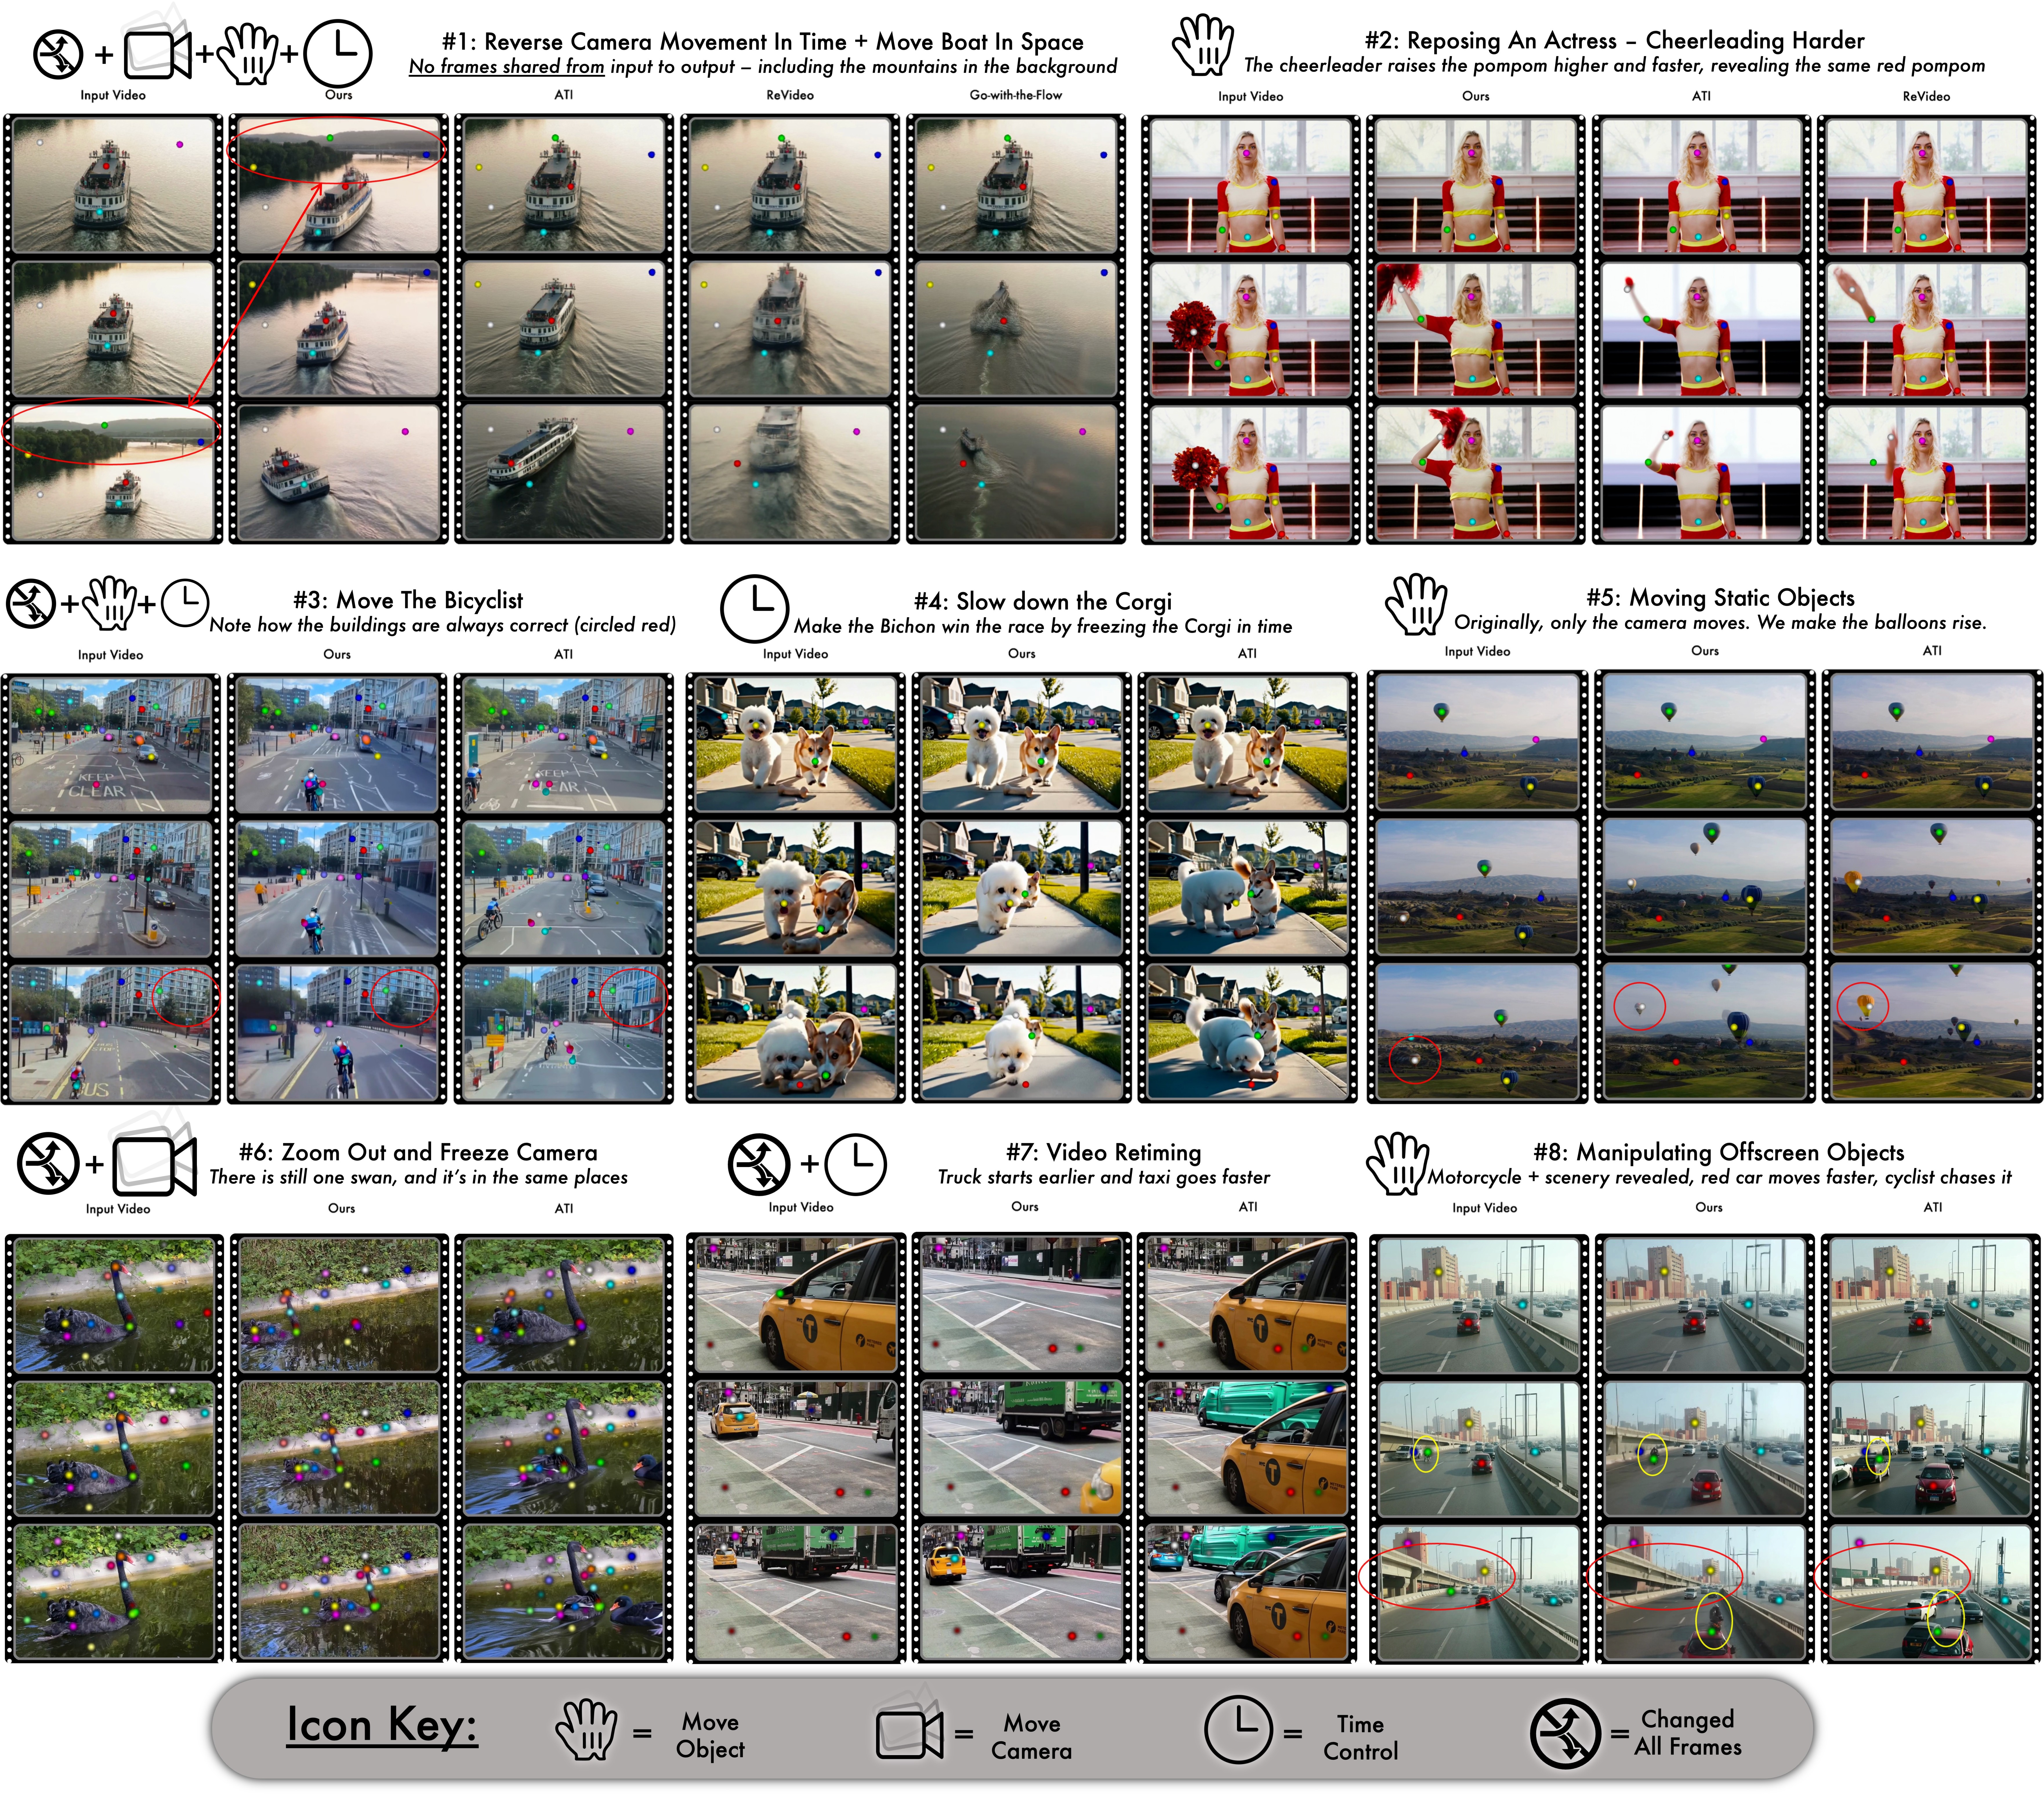
\includegraphics[width=1\linewidth]{megacomparisonfigurev2.jpg}
    % \includegraphics[width=1\linewidth]{\figfolder/MegaComparisonFigurev2}
    \caption{Comparison of our method vs.\ baselines across eight challenging motion editing scenarios.
Each row shows a different editing task with input video,
our result,
and ATI's result (with additional baselines shown for subfigure 4).
\textbf{Icon key:} Human Pose (modifying human motion),
Move Object (repositioning objects),
Move Camera (changing camera motion),
Time Control (retiming events),
Changed All Frames (no shared frames between input/output—impossible for image-to-video methods).
Colored dots track correspondence points throughout the video;
dot presence/absence indicates object visibility.
Red circles highlight key differences where baselines fail.}
    \label{fig:mega_comparison}
\end{figure*}

\noindent\textbf{Baseline comparisons.} Figure~\ref{fig:mega_comparison} compares our method against several baselines in multiple video editing scenarios, each of which demonstrate the capabilities of our motion edits. We primarily compare against ATI~\cite{ati},
a trajectory-guided image-to-video method based on WAN 2.1~\cite{wan},
our strongest baseline despite using a more powerful base model than our CogVideoX base.
Subfigure 4 additionally shows ReVideo~\cite{revideo2024} and Go-with-the-Flow~\cite{gowiththeflow2025},
which rated poorly in user evaluation—ReVideo lacks text conditioning and Go-with-the-Flow was not designed for point control.


\noindent\textbf{Edit \#1: Complex Edits on the Boat Scene.} This edit moves the boat left and shifts the camera so that mountains from the original's last frame appear in the edit's first. This requires specifying a substantial temporal trajectory change and holistic knowledge of the scene content. Ours is the only method that realistically moves the boat while correctly adjusting the camera to reveal the mountains at the beginning of the video.

\noindent\textbf{Edit \#2: Reposing a Cheerleader.} This edit raises the cheerleader's arms. The challenge involves preserving the red pom-pom, which is absent from the first frame. Ours successfully modifies the motion while retaining this content. In contrast, ATI and ReVideo rely solely on the first frame, leading to unnatural movements and a failure to preserve the pom-pom.

\noindent\textbf{Edit \#3: Move The Bicyclist.} This edit controls a cyclist visible only in the final frame of the original video. Ours correctly propagates the cyclist and tracking dots (cyan, magenta, white) throughout. ATI, lacking full temporal context, misplaces the cyclist and synthesizes wrong buildings (red circles).

\noindent\textbf{Edit \#4: Dog Race.}
Differential timing breaks single-frame-based methods. We decelerate the Corgi (green dot) to reverse the race outcome while keeping the Bichon steady. This requires independent temporal control; ATI fails to decouple the motions, incorrectly copying the Bichon and transforming a light pole into a tree.

\noindent\textbf{Edit \#5: Moving Static Balloons.}
We add upward motion to stationary balloons. The white balloon (white dot), which appears mid-video, challenges partial information methods. While ATI moves visible balloons, it renders the initially hidden white balloon orange due to missing appearance data. Our method uses full video context to maintain correct colors.

\noindent\textbf{Edit \#6: Zooming out on the Swan} 
In this DAVIS~\cite{davis2016} example, we transform a panning shot into a static, zoomed-out view. The output field of view differs entirely from the input, yet the swan must remain anchored to specific vegetation. Lacking full spatial context, ATI synthesizes a second swan and produces inconsistent motion.

\noindent\textbf{Edit \#7: Retiming a taxi.}
We do a complex isolated retiming of taxi and truck movement. This requires complete temporal understanding; ATI's single-frame generation cannot achieve this reversal. Figure~\ref{fig:mega_comparison} compares our method against ATI (WAN 2.1-based), as well as ReVideo and Go-with-the-Flow (in Subfigure 4), both of which were rated poorly due to their design limitations.

\noindent \textbf{Edit \#8: Moving an Offscreen Car.}
As the camera follows a red car, a motorcyclist enters late. We reposition this initially invisible rider behind the car while maintaining consistent background architecture. Lacking future frames to reference the rider and buildings (red circles), ATI synthesizes incorrect content.


\noindent\textbf{Discussion.}
These scenarios highlight I2V limitations: conditioning only on the first frame prevents leveraging information from the full input. Our V2V formulation enables bidirectional flow, allowing outputs to pull content from \emph{any} input frame. This handles offscreen content, camera changes, and reordering—challenges where I2V methods like ReVideo~\cite{revideo2024}, Go-with-the-Flow~\cite{gowiththeflow2025}, and MotionPrompting~\cite{motionprompt2024} fail.

% Additional comparison figures have been integrated into Figure~\ref{fig:mega_comparison}

%\begin{figure}[h]
%    \centering
%    \fullcompfig[1]{4}{\figfolder/FullComp_BlackSwan}
%    \caption{The camera is frozen while the black swan swims.}
%    \label{fig:comp_blackswan}
%\end{figure}
%
%\begin{figure}[h]
%    \centering
%    \fullcompfig[2]{5}{\figfolder/FullComp_Boat}
%    \caption{Editing the boat's trajectory and motion.\cih{todo: give categories / labels}}
%    \label{fig:comp_boat}
%\end{figure}
%
%\begin{figure}[h]
%    \centering
%    \fullcompfig[1]{4}{\figfolder/FullComp_Cheerleader}
%    \caption{Changing the motion of the cheerleader's pompoms.}
%    \label{fig:comp_cheerleader}
%\end{figure}
%
%\begin{figure}[h]
%    \centering
%    \fullcompfig[2]{4}{\figfolder/FullComp_Judge}
%    \caption{The judge walks in from the right with camera zoom.}
%    \label{fig:comp_judge}
%\end{figure}

%\begin{figure}[h]
%    \centering
%    \fullcompfig[1]{4}{\figfolder/FullComp_Candle}
%    \caption{A hand grabs the candle while the camera is stopped.}
%    \label{fig:comp_candle}
%\end{figure}

%\begin{figure}[h]
%    \centering
%    \fullcompfig[2]{4}{\figfolder/FullComp_CityBiker}
%    \caption{Editing the motion of an urban cyclist.\cih{a bit hard to see}}
%    \label{fig:comp_biker}
%\end{figure}
%
%\begin{figure}[h]
%    \centering
%    \fullcompfig[1]{4}{\figfolder/FullComp_Balloons}
%    \caption{Hot air balloons rise while the camera motion is slowed.}
%    \label{fig:comp_balloons}
%\end{figure}
%
%\begin{figure}[h]
%    \centering
%    \fullcompfig[1]{4}{\figfolder/FullComp_Dogs}
%    \caption{The corgi stays behind while the bichon moves forward.}
%    \label{fig:comp_dogs}
%\end{figure}

% \begin{figure}[h]
%     \centering
%     \includegraphics[width=1\linewidth]{\figfolder/FullComp_Shakycam}
%     \caption{Editing the camera motion on shaky footage. \cih{this just looks like brown}}    \label{fig:comp_shakycam}
% \end{figure}


\section{Conclusion}
\label{lss_sec:conclusion}

We introduce a novel language-based self-supervised learning (SSL) approach for videos, termed LSS, capable of adapting strong language-aligned image representations (CLIP \cite{radford2021clip}) to the video domain. 
In particular, we propose two self-distillation based SSL objectives, \textit{concept distillation} and \textit{concept alignment}.
Our approach trains with no video level labels or paired captions similar to prior video SSL works, but retains language alignment from image CLIP enabling direct zero-shot inference. We demonstrate state-of-the art performance in terms of linear probing with the learned representations on downstream tasks. For zero-shot operation, LSS demonstrates strong performance under both standard and transductive settings, indicating a promising direction for video SSL. 

\vspace{2em}
\noindent \textbf{Limitations, Future Work, \& Broader Impact}: 
The language alignment of LSS may be limited mostly to per-frame static information since the alignment is derived from image CLIP \cite{radford2021clip}. LSS cannot distinguish motion based categories like \texttt{"moving object left to right"}. Moreover, while containing highly discriminative and generic information at image level, CLIP features lack spatial awareness at an object level \cite{ranasinghe2022perceptual}. Our proposed model building off these representations in inherently limited in understanding object level motion and interaction within videos. However, recent progress in localization aware CLIP models \cite{ranasinghe2022perceptual,Xu2023LearningOS,xu2022groupvit} opens avenues for leveraging their object-centric or pixel-level representations to better model such video motion patterns, opening up interesting future directions. 
In terms of broader impact, the datasets and pre-trained models we use possibly contain biases, which may be reflected in LSS. However, our reduced reliance on human annotations may lower additional biases.

% % \vspace{-0.5em}
% \textbf{Reproducibility Statement}: 
% We build a codebase derived from source code of SVT \cite{Ran2021SVT} \& CLIP \cite{radford2021clip} and use pre-trained CLIP weights from \texttt{https://github.com/openai}. All experiments use publicly available datasets. Our action descriptions will be released publicly along with our codebase.

% \textbf{Acknowledgements}:
% We thank Xiang Li for helpful discussions and server setup. We also thank Kumara Kahatapitiya and Cristina Mata for helpful discussions.

\medskip

{\small
	\bibliographystyle{unsrt}
	\bibliography{neurips_2023}
}


\newpage
\section{Additional Details}

\begin{table}[t]
\centering\small
\caption[Additional Experiments with LSS]{
We report top-1 (\%) accuracy on the Kinetics-400 \cite{kinetics400} validation set for linear probing evaluation (left). All models are pre-trained on the training set of Kinetics-400 dataset. We also report a CLIP baseline for comparison purposes. Performance of our proposed approach is on-par with prior state-of-the-art and showcases improvements over our baseline method. We also report retrieval scores (top-right) for MSR-VTT and classification mAP (bottom-right) for Charades dataset.}
\vspace{0.5em}
\begin{minipage}{0.49\textwidth}
    \centering
    \setlength{\tabcolsep}{4pt}
    \scalebox{0.90}{
    \begin{tabular}{l|c|c}
    \toprule
    \rowcolor{Gray} 
    Method                                              & Backbone & Acc (\%) \\ \midrule
    CVRL \cite{qian2020spatiotemporal} \venue{(CVPR’21)}& R3D-101  & 67.6  \\
    BraVe \cite{recasens2021broaden} \venue{(ICCV'21)}  & R3D-50   & 66.7  \\ 
    Vi$^2$CLR \cite{Diba_2021_ICCV} \venue{(ICCV '21)}  & S3D      & 63.4  \\ 
    CORP \cite{Hu_2021_ICCV}        \venue{(ICCV '21)}  & R3D-50   & 66.6  \\ 
    SVT \cite{Ran2021SVT} \venue{(CVPR `22)}                              & ViT-B    & 68.1  \\ 
    VideoMAE \cite{Tong2022VidMAE} \venue{(NeurIPS `22)}                      & ViT-B    & 61.3  \\ 
    CLIP \cite{radford2021clip}                         & ViT-B    & 66.4  \\ \midrule
    LSS (ours)                                          & ViT-B    & 67.3  \\ 
    \bottomrule
    \end{tabular}}       
    \label{lss_tbl:sota_k400}
\end{minipage}
%
\begin{minipage}{0.49\textwidth}
    \centering
    \begin{tabular}{l|c|c|c} 
    \toprule \rowcolor{Gray} 
    Method & R@1  & R@5  & R@10 \\ \midrule
    CLIP \cite{radford2021clip}  & 30.6 & 54.4 & 64.3 \\
    LSS (ours)    & 33.8 & 58.2 & 70.3 \\ \bottomrule
    \end{tabular}
    
    \vspace{2em}
    
    \begin{tabular}{l|c}
    \toprule \rowcolor{Gray} 
    Method & Classification mAP \\ \midrule
    CLIP \cite{radford2021clip}  & 19.7         \\
    LSS (ours)  & 23.1         \\ \bottomrule
    \end{tabular}
\end{minipage}

\end{table}


\subsection{Prompting details}
\label{app:gpt_prompting}
Our proposed approach utilizes two sets of language based captions: categories and descriptions. While categories are obtained directly from the class labels of datasets (set of unique labels - e.g. 400 classes in Kinetics-400 dataset), the descriptions are generated automatically utilizing GPT-3 \cite{brown2020language}. For each category caption, we query GPT-3 to provide a set of descriptions and visual characteristics. 

In detail, we use the following two prompts to generate descriptions and visual characteristics:
\\
\texttt{prompt1 = "Give 4 different descriptions for the phrase: \{category\}?"} \\
\texttt{prompt2 = "List visual objects or characteristics usually seen with the action: \{category\}?"}
\\
The resulting two sets of captions are converted to text embeddings using our text-encoder, and a single average text embedding is computed. This averaged embedding is used as the description basis vector for that category. Also, the resulting dataset containing these category-description pairs is made available publicly. 


\subsection{Additional Experiments}

\noindent \textbf{Linear Probing Evaluation:}
We present more results for linear probing in \cref{lss_tbl:sota_k400} (left). Our proposed LSS improves over the baseline achieving competitive performance on Kinetics-400. 

\noindent \textbf{Text-to-video retrieval:}
An important characteristic of CLIP \cite{radford2021clip} is its retrieval ability across both language and visual modalities. In order to verify if proposed LSS retains these strengths, we run experiments on MSR-VTT text-to-video retrieval benchmark. We demonstrate how LSS improves over our baseline CLIP, reporting these results in \cref{lss_tbl:sota_k400} (top-right). 

\noindent \textbf{Charades Evaluation:}
 We explore an alternate task of zero-shot multi-label classification on the Charades video dataset. We report mAP results for this task in \cref{lss_tbl:sota_k400} (bottom-right) as an additional point of comparison.


%%%%%%%%%%%%%%%%%%%%%%%%%%%%%%%%%%%%%%%%%%%%%%%%%%%%%%%%%%%%


\end{document}